\section{Conclusions}
In this thesis, we have developed a modeling framework to better understand the propagation and onset of the SCTLD, as well as the impact of major hurricanes on transport processes over coral reefs. Our model had to be able to accurately capture ocean circulation patterns at different scales to study transport processes in the FCR. First, the large-scale Loop Current/Florida Current system had to be accurately reproduced to correctly capture its impact on eddy formation near the DRTO and the Florida Keys. Second, the model had to reproduce ocean circulation at the reef-scale to capture the recirculation and acceleration of currents between reefs and islands. This was performed by coupling the multi-scale ocean model SLIM to a connectivity-based epidemiological model (chapter \ref{chap:sctld}), a sediment transport model (chapter \ref{chap:onset}) and a spectral wave model (chapter~\ref{chap:irma}).

Our coupled hydro-epidemiological model reproduced the observed propagation of the SCTLD through the FRT by representing the transport of its causative agent within neutrally buoyant material driven by mean barotropic currents. It confirmed the results of previous ex-situ studies that showed evidence of waterborne transmission of the SCTLD with an average transmission time of the order of 10 days. Furthermore, by using coral resistance to the disease as a parameter, our model results suggested that, on average, corals had a rather low resistance against the disease. This confirmation of experimental results by model results illustrates the important potential of models to evaluate hypotheses derived from field observations on large scale systems. As such, models informed by and confronted against field knowledge \citep{foster2012connectivity} are a powerful tool to inform the management of complex ecosystems such as the FCR.

This epidemiological model was then used to build networks of potential exchanges of disease agents between $\sim 1.6\times10^4$ sub-reef areas composing the FRT during a period of three years. The analysis of these networks showed that exchanges from the Marquesas to the DRTO were interrupted during most of 2020. This interruption was likely linked to eddy activity near the DRTO and was consistent with the apparent stalling of the outbreak in the region in 2020. This confirms the role played by the Loop Current/Florida Current system in the control of the connectivity pathways in the Florida Keys and the DRTO. Furthermore, sub-reefs predicted to be more vulnerable to SCTLD in the disease networks were consistent with the observed geographic distribution of diseased corals in the DRTO. This further highlights that the modeled hydrodynamics is highly explanatory of the propagation of the disease.

The results of chapters \ref{chap:sctld} and \ref{chap:drto} show that our high-resolution biophysical model is a valuable tool to understand the spread of SCTLD in Florida. The model successfully reproduced the observed propagation of the disease in 2018-2019 and allowed us to link the observed stalling of SCTLD to observable hydrodynamic features. Furthermore, the model allowed us to deduce potential characteristics of the disease agent and its vector. This highlights the potential of biophysical models to understand the driving mechanics of ongoing marine disease outbreaks. Furthermore, metrics such as the vulnerablity and source indicators developed in chaper \ref{chap:drto} could be useful to predict and/or mitigate the spread of SCTLD in other territories of the Caribbean.

Using a sediment transport model, we investigated the impact of the PMDDP on the onset of the SCTLD outbreak in 2014. Our results suggest that the dredging operations had close to no direct impact at Virginia Key monitoring site, identified as the reef from which the disease started its propagation. However, reefs affected earlier could have been infected by chopped rock particles produced by non conventional dredging operations in the channel. Moreover, our epidemiological model suggests that disease propagation from these reefs to Virginia Key was possible. Sediments released by the PDMMP might therefore have initiated one of the worst coral disease outbreaks to date in the Caribbean. These results could have consequences on the planning of future major dredging projects in the area such as the Port Everglade Dredging Project\footnote{https://www.porteverglades.net/construction/harbor-improvements/, last consulted on February 12, 2022}. FCR is routinely suffering from important anthropogenic stresses caused by the intense activity of the area of Miami. Hence, coastal developments harm coral reefs in two ways: first, by increasing water turbidity and sedimentation during the dredging, and then by causing an increase in pollution and shipping activities. Such adverse impacts should be taken into account when planning dredging operations. The results of chapter \ref{chap:onset} suggest that the potential to initiate a coral disease outbreak should now also be taken into account when considering future dredging projects.

Finally, we developed a coupled wave-current model to study the impact of Hurricane Irma on transport processes in the Florida Keys. This coupled model correctly reproduced the observed waves and current dynamics during the passage of the hurricane. Furthermore, model results suggest that an important dissipation occurred over coral reefs through depth-induced wave-breaking and bottom friction. This important dissipation produced a large wave radiation stress gradients, which caused differences in modeled velocity of up to 1 m/s between the coupled and uncoupled model runs. However, wave-induced transport was dominated by the Stokes drift, which yielded an impact four times larger than the radiation stress gradient. Results of chapter \ref{chap:irma} strongly advocate for the use of coupled wave-currents to accurately model the dispersal of coral larvae under storm conditions. Although we built the tools to study the impact of hurricane on the exchanges of larvae between reefs by developing the coupled SLIM+SWAN model, we did not evaluate the impact of Irma on coral connectivity by lack of time.

In conclusion, we answered the four research questions defined in chapter \ref{chap:intro}:

\begin{list}{}{%
    % \setlength{\listparindent}{-0.23in}%
    \setlength{\leftmargin}{0in}%
    % \setlength{\itemindent}{-0.23in} 
    }
    \item \textbf{1. How did the \modif{stony coral tissue loss disease} spread through the \modif{Florida Reef Tract} ?}
    \begin{list}{}{\setlength{\topsep}{0pt}}
        \item The observed spread of the SCTLD through the FRT was successfully reproduced by modeling the transport of disease agents as neutrally buoyant material within the water column, and by calibrating a connectivity-based epidemiological model with field data. This therefore suggests that the disease spread through waterborne transmission. 
    \end{list}
    \item \textbf{2. What caused the apparent stalling of the propagation of \modif{disease} ?}
    \begin{list}{}{\setlength{\topsep}{0pt}}
        \item Our results suggest that there was an interruption of hydrodynamic-driven exchanges from the Florida Keys and the Marquesas to the DRTO during most of 2020, which prevented the propagation of disease agents westward. This interruption of the disease connectivity pathways to the DRTO was likely related to the local eddy activity generated by the meandering of the Florida Current.
    \end{list}
    \item \textbf{3. What was the impact of the \modif{PortMiami Deep Dredge Project} on the onset of the \modif{disease outbreak}?}
    \begin{list}{}{\setlength{\topsep}{0pt}}
        \item Modeling of sediment transport suggests that the chopped rock particles produced by the non conventional dredging activities reached reefs where signs of disease were first reported during the first half of 2014. Furthermore, the modeled disease connectivity suggested that disease propagation from these sites to Virginia Key was possible prior to September 2014. The sediments released by the PMDDP might thus have triggered the onset of the SCTLD outreak at this site.
    \end{list}
    \item  \textbf{4. What is the effect of hurricane-induced wave-current interactions on transport processes and should they be taken into account when modeling the dispersal of coral larvae ?}
    \begin{list}{}{\setlength{\topsep}{0pt}}
        \item Results of a coupled wave-current model suggest that wave-induced transport under storm conditions, dominated by Stokes drift, can yield differences in particle trajectories of up to 20 km. Wave-current interactions should thus be taken into account to accurately model the dispersal of coral larvae during hurricanes.
    \end{list}
\end{list}

\modif{\section{Our contribution to the model development}}

\modif{Answering the aforementioned research questions required the development of new modeling tools. As this thesis relied heavily on Lagrangian transport modeling, several features were added to SLIM's particle tracker. Although the transport of the particles in itself was already implemented in the model, we developed new model features to characterize the state of the particles and compute new connectivity indicators. The particle state can be used to represent biological traits such as the competency of coral larvae or abiotic characteristics such as the decay rate of diseased agent mass or the diameter of sediment particles. Post-processing features were developed to compute the concentration of suspended and deposited particles. We also developed tools to derive connectivity indicators such as the shortest paths between a pair sub-reef polygons in the connectivity networks. Additionally, we developed an epidemiological model using the computed connectivity matrices to simulated the spread of the stony coral tissue loss disease throughout Florida's Coral Reef. Finally, the particle tracker was made more flexible by developing new readers for different ocean model outputs such as HYCOM or the Nucleus for European Modelling of the Ocean (NEMO; \citealp{madec2017nemo}).}

\modif{Additionally, coupling SLIM with SWAN required some modifications of SLIM. First, we implemented a new parameterization of the wind drag coefficient to account for the formation of spume at the ocean-atmosphere interface in heavy wind conditions. An additional term was also added to the model's equations to account for the gradient of atmospheric pressure generated at the center of the hurricane. Using SWAN also required the implementation of tools to process the wave spectrum and the associated parameters in SLIM. The implementation of the coupling between the two models followed the same approach as the ADCIRC+SWAN model. It required the development of tools to convert SLIM outputs and forcing into SWAN format, and to allow SLIM to read SWAN outputs. Compared to ADCIRC+SWAN, an additional challenge that we had to overcome was the fact that SLIM is based on discontinous Galerkin finite element models while SWAN requires continuous fields on the mesh. This was especially critical when defining the communication between the nodes of the partitions of SWAN based on the partitioning of the mesh used in SLIM.}

\modif{However, the implementation of the coupling could be improved, as the two models are currently alternatively run and stopped with different initial and boundary conditions. The coupling therefore induces unwanted initialization computational costs each time one of the two model is run. Suppressing these initialization costs would strongly reduce the overhead of the coupling. Furthermore, a strong limitation of the coupled model is the temporal complexity of SWAN, which runs four times slower than SLIM. A way to tackle this issue would be to run SWAN on a smaller, coarser mesh than SLIM to reduce its computation time at the expense of a potentially reduced resolution in the wave outputs. Alternatively, as robust estimates of the Stokes drift can be derived from the surface wind speed \citep{ardhuin2009observation}, a one-way coupled wave-current model could be developed using the vortex force formalism. In such a model, wave impact on currents would be modeled in SLIM through interactions between a wind-parameterized Stokes drift and the vorticity of the modeled currents, as in \cite{curcic2015explicit}.} \newline

\section{Perspectives for future works}

\subsection*{Combining disease and larval connectivity}
All chapters dedicated to SCTLD rely on the concept of connectivity. In this context, connectivity negatively impacts coral reefs as it drives the propagation of disease agents. However, connectivity is actually a double-edged sword. Larval connectivity promotes the resilience of the reef network as it allows the recolonization of disturbed reefs following extreme events such as mass bleaching, hurricanes or disease outbreaks. Larval connectivity is therefore a valuable tool to inform coral reef protection and restoration \citep{botsford2009connectivity,mumby2011reserve}. Identifying reefs that are both good sources and sinks of larvae in the connectivity network indicates the optimal sites for coral outplants in the context of active restoration. Furthermore, knowledge about larval connectivity would allow us to build robust and sustainable networks of connected marine protected areas. As SLIM allows the computation of larval connectivity \citep{thomas2014numerical,frys2020fine,figueiredo2021global}, a possible application of the tools developed in this thesis is the combination of both types of connectivity.  This combined information would allow us to identify reefs that are good larval sources and have low vulnerability to the disease. A possible measure of larval supply to the network is the (weighted) out-degree of reefs in the larval connectivity network, as reefs with strong and numerous outgoing connections in the network are more likely to send many larvae to many connected reefs. Vulnerability to disease can be evaluated using the (weighted) in-degree of reefs in the disease connectivity network, as reefs with strong and numerous incoming connections are more likely to receive more disease agents from many connected reefs. Therefore, reefs with high restoration potential would correspond to reefs with large larval (weighted) out-degree and low disease (weighted) in-degree. This approach has been applied in \cite{holstein2022} and could be further developed in future studies using more complex connectivity metrics such as the PageRank index \citep{frys2020fine}. 

\subsection*{Improving the epidemiological model}
A limitation of the epidemiological model developed in chapter \ref{chap:sctld} is that it uses species-averaged parameters and assumes an uniform distribution of coral species throughout the FRT. The fact that our model correctly reproduced the observed spread of SCTLD for a well-defined range of values of coral resistance to the disease highlights the important impact of this parameter on the propagation of the disease. However, coral susceptibility to SCTLD can significantly vary between species and ranges from highly susceptible (\eg~\textit{Dichocoenia stokesii}, \textit{Meandrina meandrites}) to intermediately susceptible (\eg~\textit{Orbicella faveolata}, \textit{Montastrea cavernosa}) and weakly susceptible (\eg~\textit{Acropora Palmata}, \textit{Acropora cervicornis}). A first improvement could therefore be to consider classes of corals with different susceptibilities and hence use different infection and removal parameter values in the model. Such a development could require the use of more advanced graph theory tools such as multilayer networks \citep{kivela2014multilayer,pilosof2017multilayer}. Furthermore, this improvement would increase the number of variables and parameters of the model, which  would make its calibration more complex. Moreover, this new modeling framework would require estimates of the distribution of the different coral species across the FRT. Compiling this data and deriving realistic estimates would represent a significant challenge. Interestingly, adding species-specific or location-specific parameters in the model would also allow the evaluation of the impact of disease mitigating actions. Lesion treatment using antibiotics could for instance be taken into account in the model by locally reducing the transmission and/or removal parameters. The model parameters could also be made time-dependent as SCTLD progression was reported to slow down during warmer months in the US Virgin Islands \citep{meiling20203d}. Another improvement would be the inclusion of additional processes in the model. For instance, reinfection by SCTLD is currently not possible as corals are "removed" once they are affected by the disease. Given the high mortality of the disease, the "removed" state of the model was assumed equivalent to "dead". However, one might want to discriminate between coral recovery and mortality. Yet, again, adding processes implies an increase in the number of parameters to be calibrated. These modifications could lead to an endemic disease dynamics. 

\modif{\subsection*{Better understanding the impact of hurricanes on corals}}
\modif{In this thesis, the impact of hurricanes on coral reef ecosystems was mostly evaluated by modeling wave-induced advective transport processes. However, when studying the propagation of drifting particles, assessing the impact of hurricanes on the diffusion (\ie~spread) of the particle cloud is also of interest. This could be performed by computing the distance between the positions of the particles of the cloud and its center of mass or by evaluating the evolution of the concentration of particles in the cloud. Furthermore, wave-induced transport is not the only way tropical cyclones affect coral reef biota. First, they can cause a wholesale destruction of the reefs as they pass over them. However, this destruction can sometimes have positive consequences by facilitating asexual recruitment and cleaning algal overgrowth on the reefs \citep{banks2008reef}. Moreover, water mixing and upwelling by hurricane can reduce water temperature and alleviate the thermal stress experienced by corals \citep{wilkinson2008status}. Furthermore, hurricanes increase water turbidity and induce coral burial by resuspending sediments. These impacts could be assessed by combining the developed coupled wave-current model with our sediment transport model. Moreover, hurricane interact with the Florida Current by disrupting its vertical structure and reducing its transport \citep{oey2007hurricane}. These structural perturbations might have consequences on eddy activity near the Florida Keys and therefore impact nutrient concentration and larval recruitment in the region \citep{lee1992influence}. Our study could therefore be extended by evaluating the impact of Hurricane Irma on the ocean state and the broader circulation patterns in Florida although baroclinic models might be required. Finally, by modifying the ocean circulation on their passage, hurricanes might influence the connectivity of the Florida Reef Tract. The coupled SLIM+SWAN model could thus be used to evaluate the impact of Hurricane Irma on coral larval connectivity as a continuation of the work initiated in chapter \ref{chap:irma}. Furthermore, the hurricane-induced transport might have impacted the propagation of SCTLD through Florida's Coral Reef. Hurricane Irma could therefore have acted as a "super spreader" of disease agents or as a barrier to the propagation of the outbreak. This effect could be investigated by combining SLIM+SWAN with the developed epidemiological model.} \newline

\subsection*{Better understanding the protective role of corals against storm waves}
Simulation results from the coupled wave-current model suggest that storm waves were significantly dissipated over reefs. The modeled significant wave height under the center of the hurricane reduced from 8 m to $<1$ m over the barrier reef during the passage of the hurricane (Fig. \ref{ccl:swh}). This highlights the important protective role of coral reefs against coastal flooding hazard. Better understanding this role can motivate coral reef restoration efforts. For instance, \cite{ferrario2014effectiveness} estimated that coral reefs could provide wave attenuation comparable to artificial defenses such as breakwaters for a much lower cost. However, modeling the wave-flow dynamics at the reef scale is particularly challenging and requires models that can explicitly represent small-scale nonhydrostatic processes. The smallest scales that models such as SLIM and SWAN can simulate is limited by the intrinsic assumptions in the model formulations, i.e., hydrostatic for SLIM and phase-averaged for SWAN. These assumptions are no longer valid as soon as the horizontal scales of motion become comparable to the vertical scales \citep{marshall1997hydrostatic}. For such situations, it becomes necessary to couple the SLIM+SWAN model with a phase-resolving nonhydrostatic wave-flow model, hence achieving a multi-physics modeling framework. Nonhydrostatic models are more expensive to	 run as they require a much finer spatial resolution of the order of a meter and have a more complex physics. They can therefore often be used only in rather small areas and over short periods of time \citep{fringer2019future}. One promising approach to tackle this issue would be to use machine learning algorithms to locally emulate the dynamics of a complex high-resolution model and hence speed up the computational process \citep{kasim2021building}. Machine learning is based on the principle of extracting information from data, which can either be observational data or high-resolution model outputs, and deriving relationships between datasets without the need for physics-based models. This procedure has recently been applied to ocean modeling and was able to reproduce the temporal and spatial variability of unresolved turbulent processes, when given a smoothed view of the dynamics \citep{bolton2019applications}. Additionally, this multi-physics modeling frameworks could be used to better capture the motion of coral larvae over reef. This would improve the modeled coral connectivity, as the initial motion of larvae over reefs then drives larval transport following mass spawning events, and initiates coral connectivity. 

\begin{figure}
	\centering
	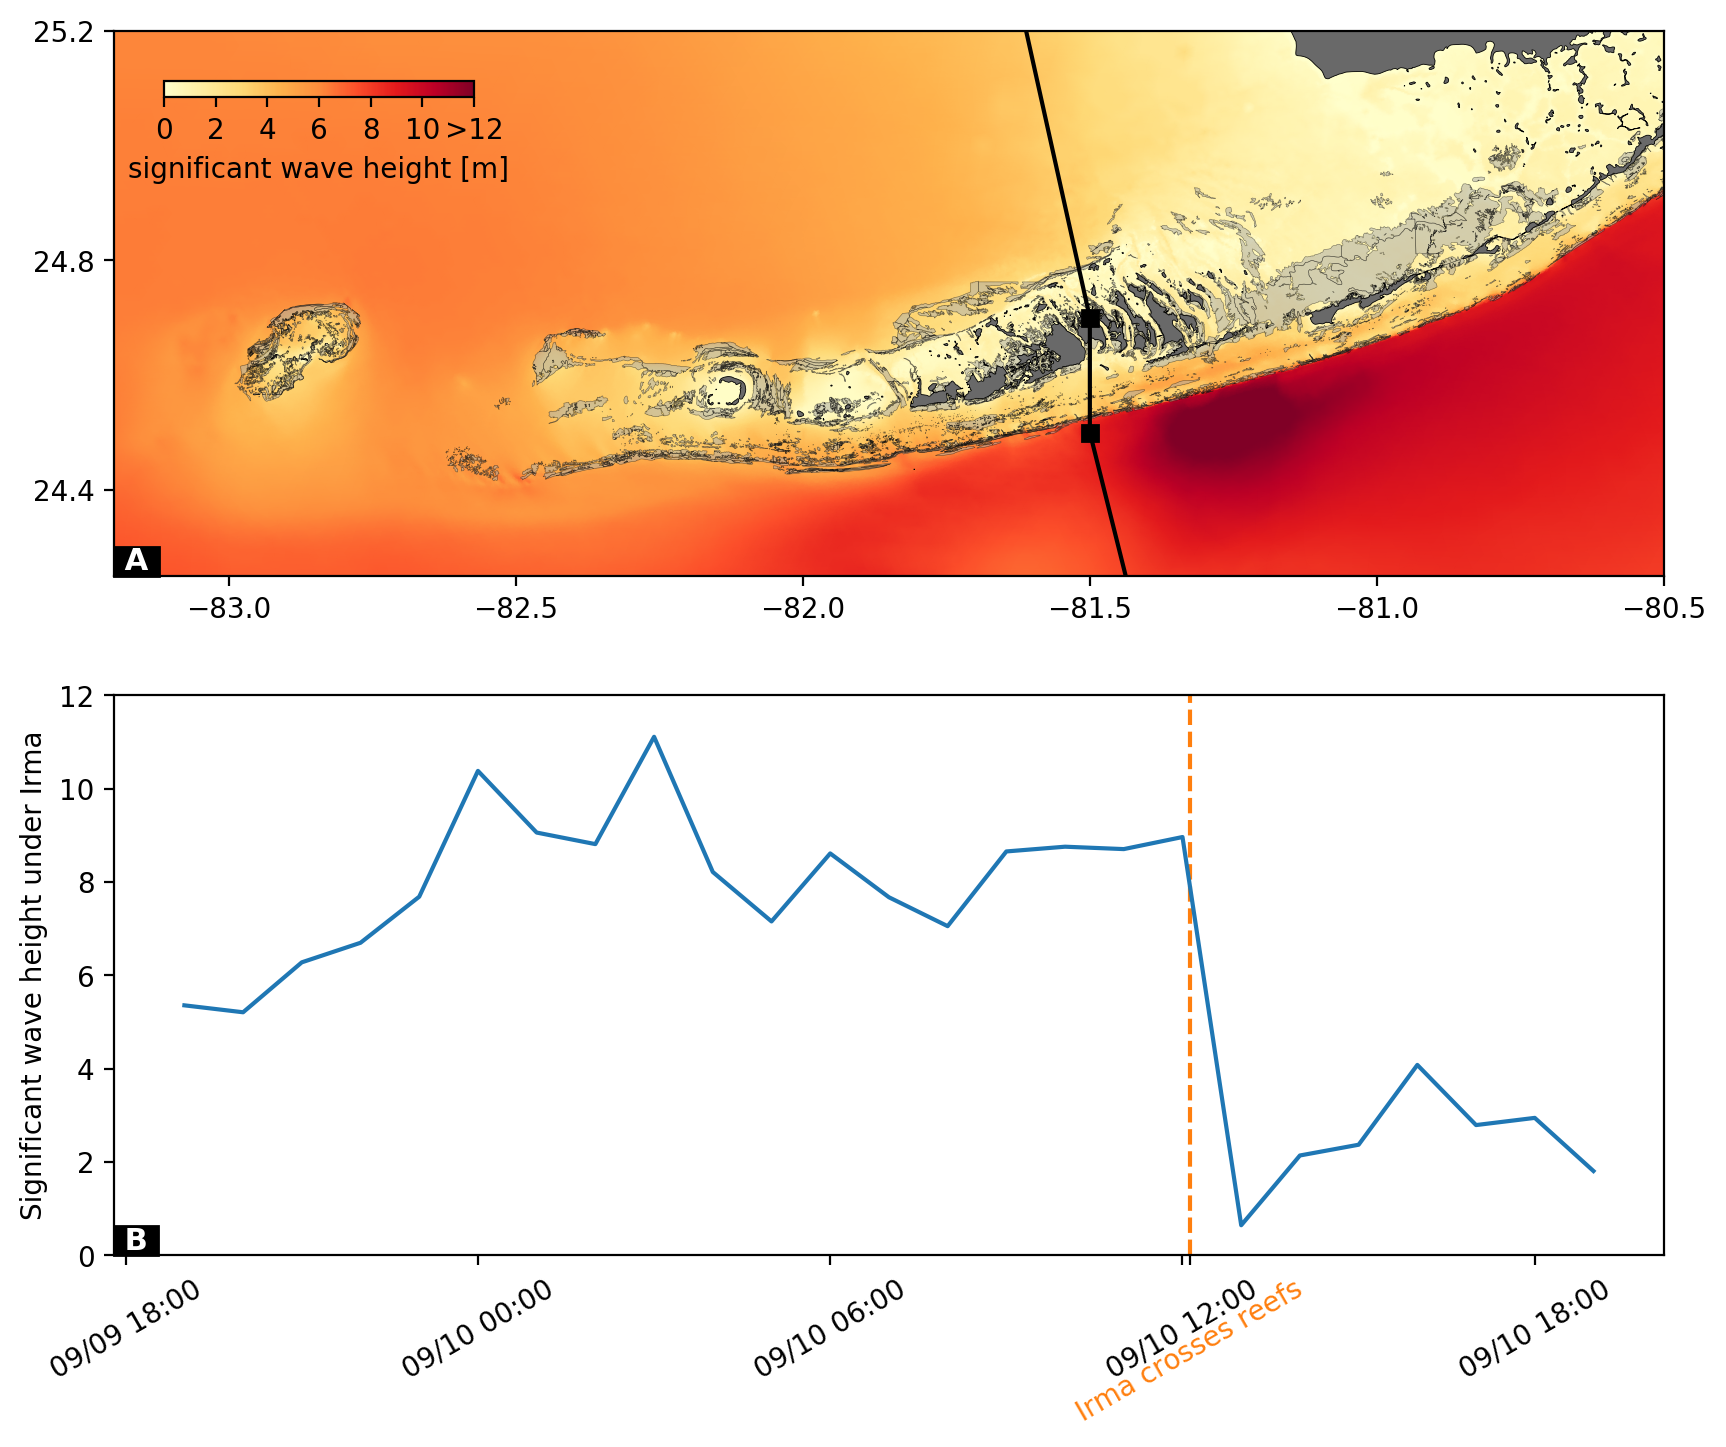
\includegraphics[width=\textwidth]{chapters/conclusions/figures/swh_curve.png}
	\caption{\textbf{A}: Snapshot of the significant wave height modeled by the coupled SLIM+SWAN model during Hurricane Irma, on Sept 10, 2017 at 1200 UTC. The path of the hurricane is shown by a black line with squares. Land is shown in dark gray and reefs in light gray. \textbf{B}: Evolution of the significant wave height under the center of Irma. Important wave attenuation is visible between the fringing coral reefs and the islands.}
	\label{ccl:swh}
\end{figure}


% Last nice chapter
The work presented in this thesis has demonstrated the capabilities of modeling tools to inform the management of Florida's Coral Reef. Models allow the evaluation of hypotheses derived from field observations on large-scale systems and can help infer the characteristics and underlying mechanisms of complex processes. Furthermore, they can be used in a predictive manner to evaluate the impacts of changing environmental conditions on a given ecosystem. Additionally, the framework developed in this thesis relies on the same widely used tools as larval transport models. Both approaches could thus be easily combined to optimize the design of coral reef protection and restoration campaigns. The development of such modeling tools coupled with field an lab studies may thus inform reef management to maintain the biological functions of coral reefs through the Anthropocene.